% Autor: Leonhard Segger, Alexander Neuwirth
% Datum: 2017-10-30
\documentclass[
	% Papierformat
	a4paper,
	% Schriftgröße (beliebige Größen mit „fontsize=Xpt“)
	12pt,
	% Schreibt die Papiergröße korrekt ins Ausgabedokument
	pagesize,
	% Sprache für z.B. Babel
	ngerman
]{scrartcl}

% Achtung: Die Reihenfolge der Pakete kann (leider) wichtig sein!
% Insbesondere sollten (so wie hier) babel, fontenc und inputenc (in dieser
% Reihenfolge) als Erstes und hyperref und cleveref (Reihenfolge auch hier
% beachten) als Letztes geladen werden!

\usepackage{tikz}
\usetikzlibrary{calc,patterns,angles,quotes} % loads some tikz extensions\usepackage{tikz}
\usetikzlibrary{babel}

% Silbentrennung etc.; Sprache wird durch Option bei \documentclass festgelegt
\usepackage{babel}
% Verwendung der Zeichentabelle T1 (Sonderzeichen etc.)
\usepackage[T1]{fontenc}
% Legt die Zeichenkodierung der Eingabedatei fest, z.B. UTF-8
\usepackage[utf8]{inputenc}
% Schriftart
\usepackage{lmodern}
% Zusätzliche Sonderzeichen
\usepackage{textcomp}

% Mathepaket (intlimits: Grenzen über/unter Integralzeichen)
\usepackage[intlimits]{amsmath}
% Ermöglicht die Nutzung von \SI{Zahl}{Einheit} u.a.
\usepackage{siunitx}
% Zum flexiblen Einbinden von Grafiken (\includegraphics)
\usepackage{graphicx}
% Abbildungen im Fließtext
\usepackage{wrapfig}
% Abbildungen nebeneinander (subfigure, subtable)
\usepackage{subcaption}
% Funktionen für Anführungszeichen
\usepackage{csquotes}
\MakeOuterQuote{"}
% Zitieren, Bibliographie
\usepackage{biblatex}
% Zur Darstellung von Webadressen
\usepackage{url}
%chemische Formeln
\usepackage[version=4]{mhchem}
% siunitx: Deutsche Ausgabe, Messfehler getrennt mit ± ausgeben
\usepackage{floatrow}
\floatsetup[table]{capposition=top}
\usepackage{float}
% Verlinkt Textstellen im PDF-Dokument
\usepackage[unicode]{hyperref}
% "Schlaue" Referenzen (nach hyperref laden!)
\usepackage{cleveref}
\sisetup{
	locale=DE,
	separate-uncertainty
}
%\bibliography{14Mo_O4_25-06-2018_References}

\begin{document}
	
	\begin{titlepage}
		\centering
		{\scshape\LARGE Versuchsbericht zu \par}
		\vspace{1cm}
		{\scshape\huge O4 - Magneto-Optischer Kerr-Effekt \par}
		\vspace{2.5cm}
		{\LARGE Gruppe 14Mo \par}
		\vspace{0.5cm}
		
		{\large Alexander Neuwirth (E-Mail: a\_neuw01@wwu.de) \par}
		{\large Leonhard Segger (E-Mail: l\_segg03@uni-muenster.de) \par}
		\vfill
		
		durchgeführt am 25.06.2018\par
		betreut von\par
		{\large Marcel Holtmann}
		
		\vfill
		
		{\large \today\par}
	\end{titlepage}
	\tableofcontents
	\newpage

	\section{Kurzfassung}
	Es wird der Magneto-Optischer Kerr-Effekt genutzt, um die Hysteresekurve einer ferromagnetischen Probe zu bestimmen.
	Dieser sorgt für eine Polarisationsrichtungsänderung von an der Probe reflektiertem Licht, die proportional zur Magnetisierung der Probe ist, weshalb er eine Bestimmung der Magnetisierung in Abhängigkeit vom angelegten Magnetfeld erlaubt.
	
	Zunächst wird angenommen, dass die magnetische Flussdichte des Magnetfelds, dass von zwei Spulen zwischen zwei Polschuhen aufgebaut wird, proportional zum durch die Spulen fließenden Spulenstrom ist.
	Dies kann innerhalb der Messungenauigkeiten eindeutig bestätigt werden.
	
	Dann wird untersucht, ob die Messung der Intensität eines durch einen Analysator transmittierten, an der Probe reflektiertem, linear polarisierten Laserstrahls die Messung der charakteristischen symmetrischen Hysteresekurve einer Probe aus einem Cobalt/Platin-Schichtsystem erlaubt.
	Dies kann bestätigt werden und beispielhaft wird gezeigt, welche Faktoren einen störenden Einfluss auf die Messung haben können. %TODO Zu sehr Misserfolge in Erfolge umgebogen? ca. 130 Wörter
	%TODO Zahlenwerte, gibt halt nur den 0,03T, wäre halt füll Material und man kann nemmer sagn, dass wir keine Werte haben auch wenns eig. halt wasted ist.
	
	\section{Methoden}
	In \cref{fig_aufbau} ist der Versuchsaufbau dargestellt.
	Dabei befindet sich eine Probe aus einem Cobalt/Platin-Schichtsystem in einem Magnetfeld, das von zwei Spulen zwischen zwei Polschuhen aufgebaut wird.
	Zunächst wird das Magnetfeld am Ort der Probe in Abhängigkeit vom durch die Spulen fließenden Strom gemessen, indem anstelle der Probe eine Hall-Sonde zwischen die Polschuhe gebracht wird.
	Diese wird in einem Winkel von ca. \SI{45}{\degree} zur Strecke, die die Polschuhe verbindet, positioniert, da eine Messung parallel zur Magnetfeldrichtung aufgrund der Position der Polschuhe nicht möglich ist.
	Dazu wird der Strom von \SIrange{0}{1}{\ampere} in \SI{0,05}{\ampere} Schritten erhöht.
	Dies wird dann bei umgekehrter Flussrichtung wiederholt. %TODO würde ich kürzen und halt -1 bis 1

	Dann wird die Probe zwischen die Polschuhe gebracht und ein Laser durch einen Polarisationsfilter, der den Strahl senkrecht linear polarisiert, auf die Probe gerichtet.
	Ein weiterer Polarisationsfilter wird als Analysator mit einem Polarisationswinkel von \SI{45}{\degree} zum Polarisator in den reflektierten Strahl gebracht, weil gemäß dem Gesetz von Malus die Intensität proportional zum quadrierten Kosinus des Differenz der Polarisationswinkel ist und die Ableitung des quadrierten Kosinus bei einem Winkel von \SI{45}{\degree} maximal ist. %hat der Typ behauptet, ist glaub ich nicht true ¯\_(ツ)_/¯, ich denke auch 50/50
	Daher maximiert dies die Messgenauigkeit.
	Ein Lichtsensor wird so aufgestellt, dass der Strahl in ihm endet.%TODO Ich finde es relevant zu erwähnen, dass wir die beim Messen der Hysterese bei MAximum/Miniumum Magnetfeld anfangen, also das Mittelding vom Ursprung net gibt.
	
	Die vom Lichtsensor gemessene Intensität wird in Abhängigkeit vom Spulenstrom aufgenommen.
	Dabei ist der Raum durch einen Vorhang abgedunkelt und der Strom wird wie zuvor in beiden Flussrichtungen schrittweise erhöht.
	Alle Messungen wurden bei Raumtemperatur durchgeführt.
	
	\begin{figure}[H] 
		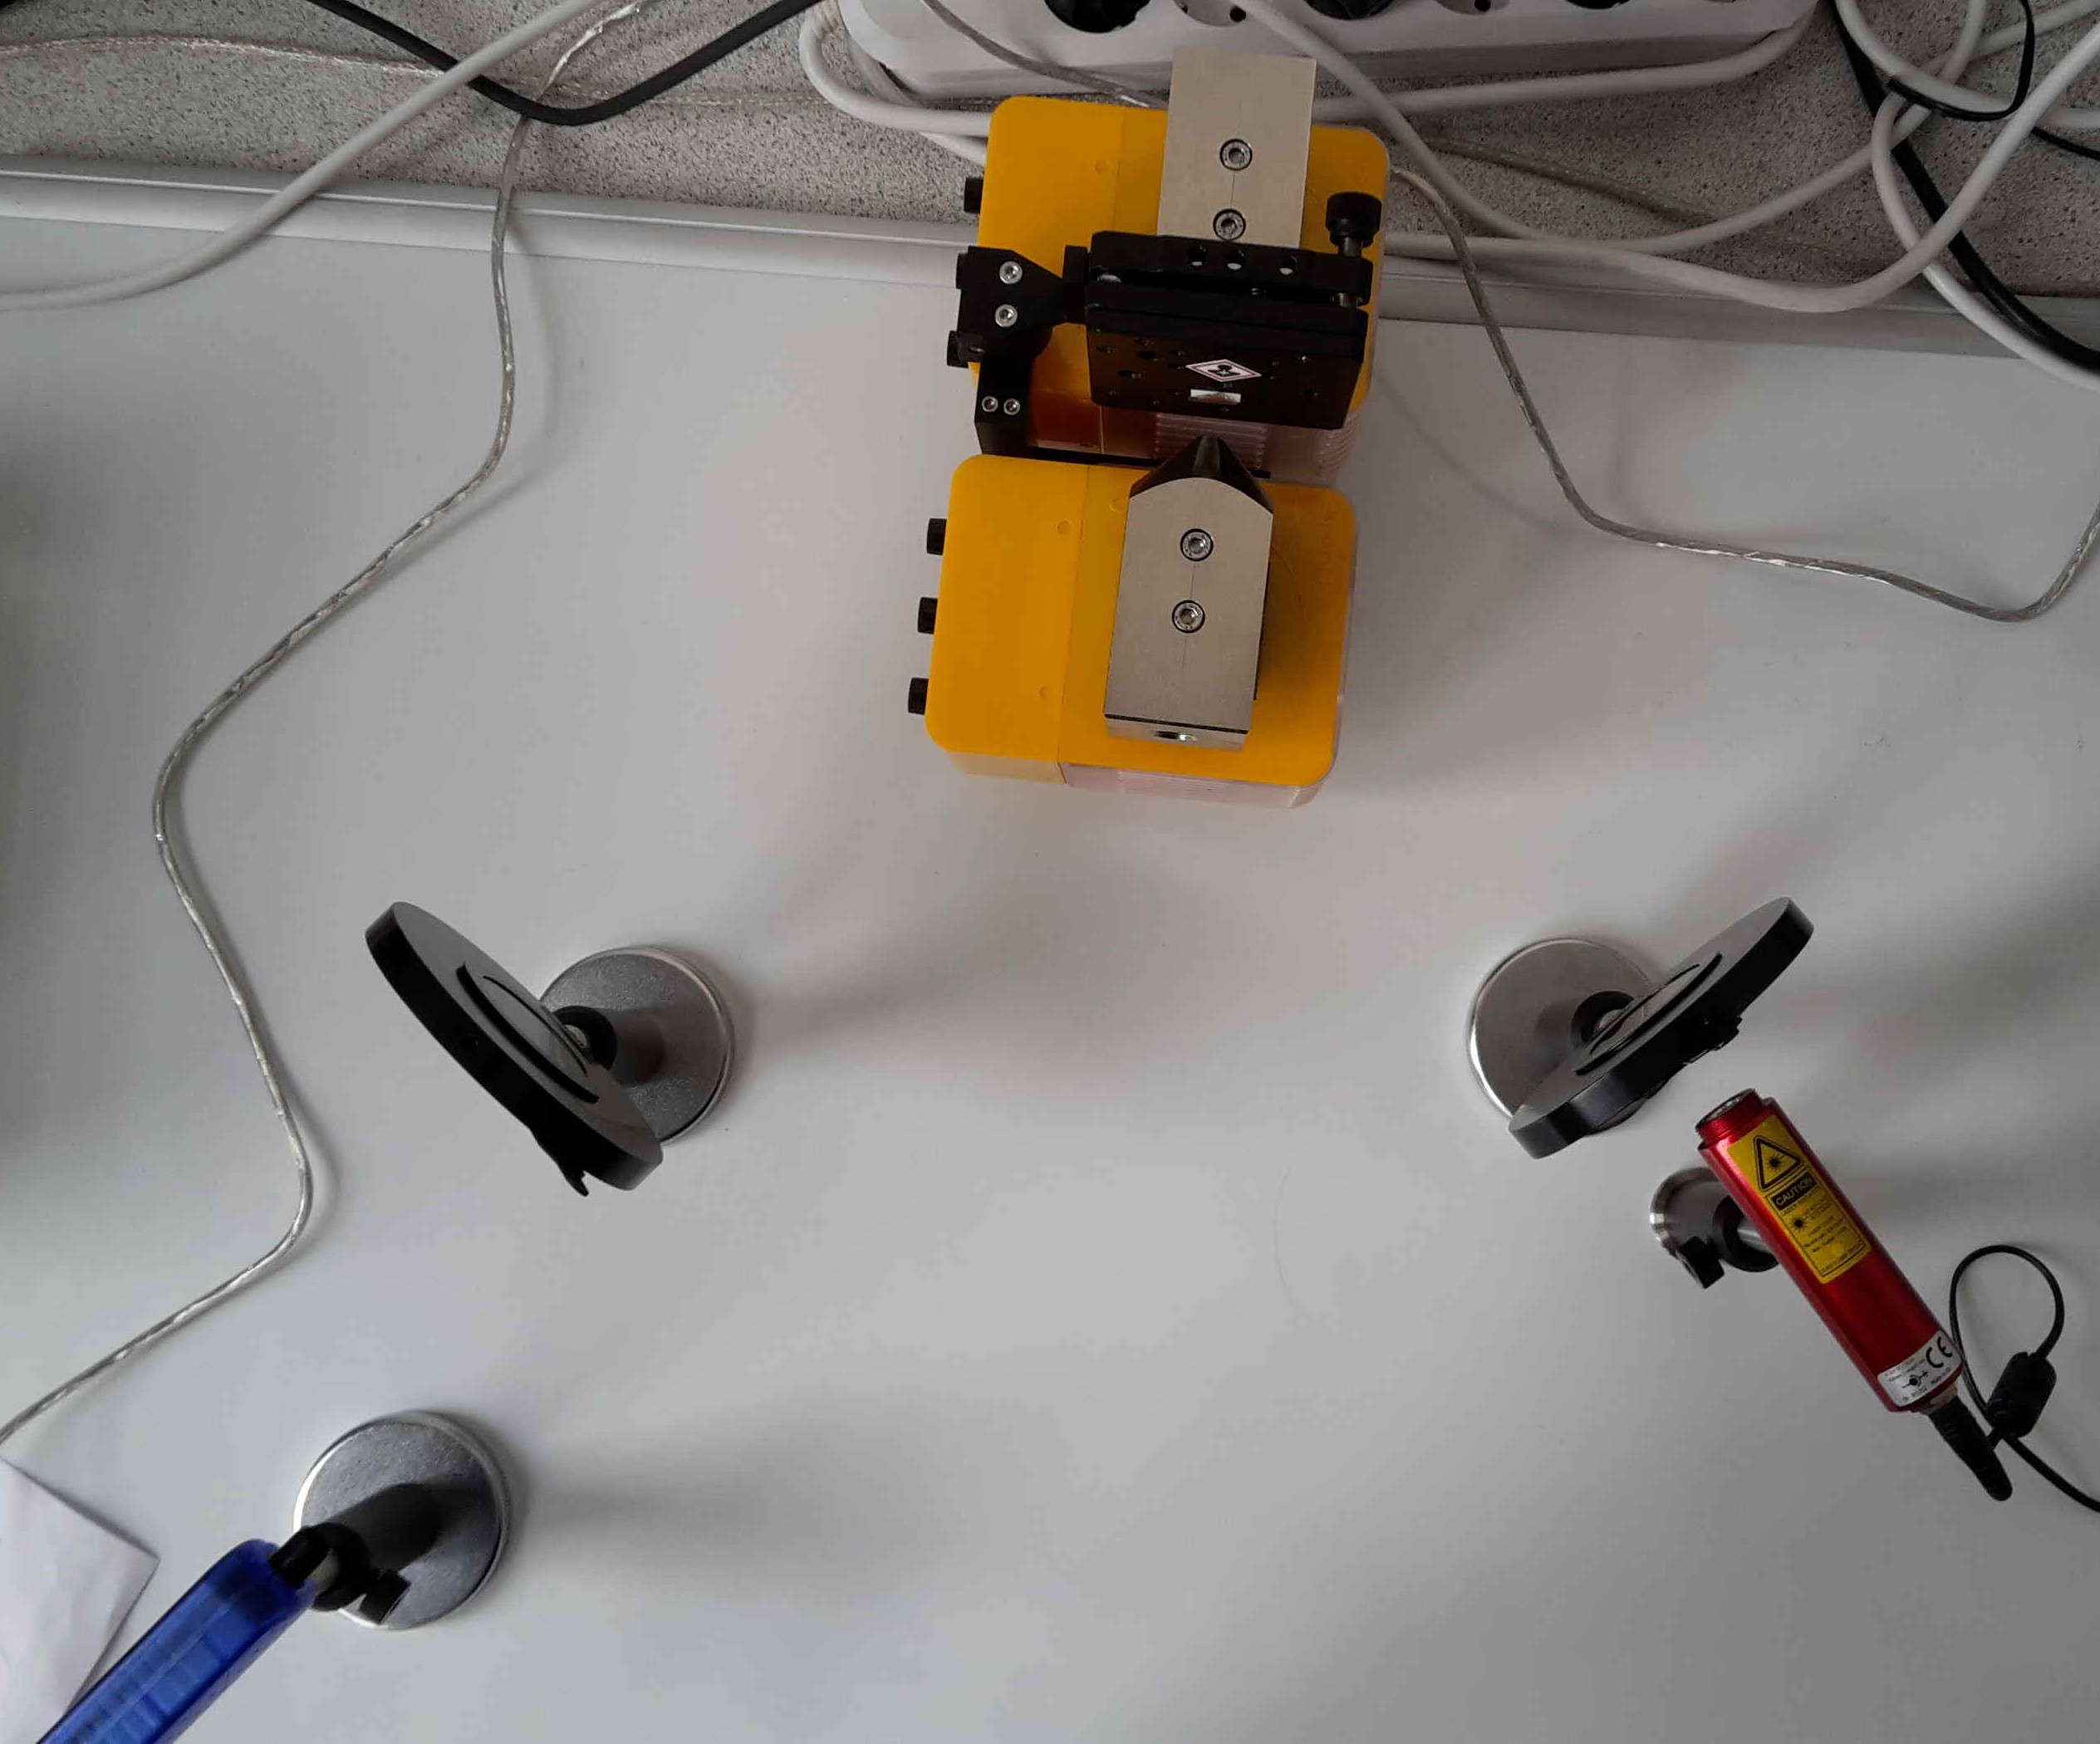
\includegraphics[width=0.7\textwidth]{O4_Aufbau} %TODO größe anpassen am Ende
		\centering
		\caption{Darstellung der für das Experiment verwendeten Elemente. Ein linear polarisierter Laserstrahl trifft auf eine Probe aus einem Cobalt/Platin-Schichtsystem, die sich in einem Magnetfeld befindet. Der reflektierte Strahl trifft durch einen Polarisationsfilter in einen Lichtsensor. Aus Übersichtsgründen sind keine Kabel an die Spulen angeschlossen. Die optischen Komponenten sind im Bild nicht justiert.} 
		\label{fig_aufbau}
		\centering
	\end{figure}
	
	\section{Ergebnisse und Diskussion}
	%TODO Unsicherheiten
	

	\subsection{Beobachtung und Datenanalyse}
	%TODO Einflüsse von veränderten Parametern auf Messung
	\subsubsection{Unsicherheiten} %TODO GGF IN DATENANYLSY
	Die Unsicherheiten werden gemäß GUM ermittelt. 
	Außerdem wird für Unsicherheitsrechnungen die Python-Bibliothek "uncertainties" verwendet.
	\begin{description}
		\item[Amperemeter/Multimeter:] Der Messwert des Betriebsstroms der Spulen wird von einem Multimeter abgelesen. 
			Dieses zeigt die Stromstärke auf zwei Nachkommastellen genau an. 
			Es ergibt sich also eine Unsicherheit von \SI{3}{mA} (rechteckige WDF).
			Dabei wird angenommen, dass der eigentliche Messfehler des Gerätes dem Displayfehler gegenüber verschwindet. 
		\item[Hall-Sonde:]  Die Stärke des Magnetfelds wird mit einer Hall-Sonde gemessen. Die Messwerte schwanken in der fünften Nachkommastelle, sodass eine Unsicherheit von \SI{30}{\mu T} angenommen wird (rechteckige WDF).
		\item[Photodiode:]  Die relative Intensität des Lichts wird mit einer Photodiode gemessen. Die Unsicherheit bei dieser Messung wird mit \SI{0,1}{} abgeschätzt (rechteckige WDF).
		\item[Geodreieck:]  Die Winkelmessung ließ sich aufgrund der Geometrie der Polschuhe nur ungenau durchführen, weshalb eine Unsicherheit von \SI{2}{\degree} angenommen wird (dreieckige WDF).
	\end{description} 

	\subsubsection{Bestimmung des Magnetfelds}
	\label{ss_spule}
	Die Stärke des Magnetfelds an der Position der Probe wird mit der Hall-Sonde in einem Winkel $\theta$ gemessen.
	Bei $\theta=\SI{90}{\degree}$ wurde $B_\text{Mess} = \SI{0,1}{mT}$ gemessen.
	In \cref{fig_draw} sind die Winkelverhältnisse dargestellt. 
	$\vec B$ ist das Magnetfeld senkrecht zur Probenoberfläche. 
	$\vec B_\text{Hall}$ zeigt die Messrichtung der Hall-Sonde an.
	Der Messwert $ B_\text{Mess}$ ist die Projektion von $\vec B$ auf $\vec B_\text{Hall}$:
	\begin{equation}
		B_\text{Mess}  = \vec B \cdot \frac{\vec B_\text{Hall}}{\left| B_\text{Hall} \right|} = \left| B \right| \cdot \cos(\theta)
	\end{equation}
	Mit $\theta=\SI{45\pm 2}{\degree}$ folgt also $B = (\sqrt{2}\pm0,05) \cdot B_\text{Mess}$.

	\begin{figure}[H]
		\centering
		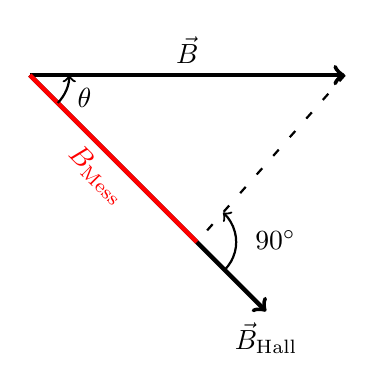
\begin{tikzpicture} %dafuq, ziemlich nice
			\coordinate (ori) at (0,0);
			\coordinate (mag) at (4,0);
			\coordinate (hall) at (3,-3);
			\coordinate (senk) at (2.12,-2.12);

			\draw[->, ultra thick] (ori) -- (mag) node [pos=.5,sloped,above] {$\vec B$};
			\draw[->,ultra thick] (ori) -- (hall) node [sloped,below] {$\vec B_\text{Hall}$};
			\draw[-,ultra thick,color=red] (ori) -- (senk) node [pos=.5,sloped,below] {$B_\text{Mess}$};
			\draw[loosely dashed, thick] (mag) -- (senk) node [pos=.5,sloped,above] {};
			\pic[draw, ->, thick, angle eccentricity=1.5,"$\theta$"] {angle = hall--ori--mag};
			\pic[draw, ->, thick, angle eccentricity=2.0,"$\SI{90}{\degree}$"] {angle = hall--senk--mag};
		\end{tikzpicture}
		\caption{Skizze zur Veranschaulichung der Messung des Magnetfelds in Abhängigkeit vom Stromfluss durch die Spulen.}
		\label{fig_draw}
	\end{figure}
	
	Die Messergebnisse sind in \cref{fig_spule} dargestellt. 
	Da ein linearer Zusammenhang erwartet wird, wird ein linearer Fit berechnet.
	Der y-Achsenabschnitt $b$ ist vernachlässigbar klein, sodass sich als Proportionalitätsfaktor zwischen Stromstärke und Magnetfeld $a= \SI{-0,0532+-0,0001}{T/A}$ ergibt.
	\begin{figure}[H] 
		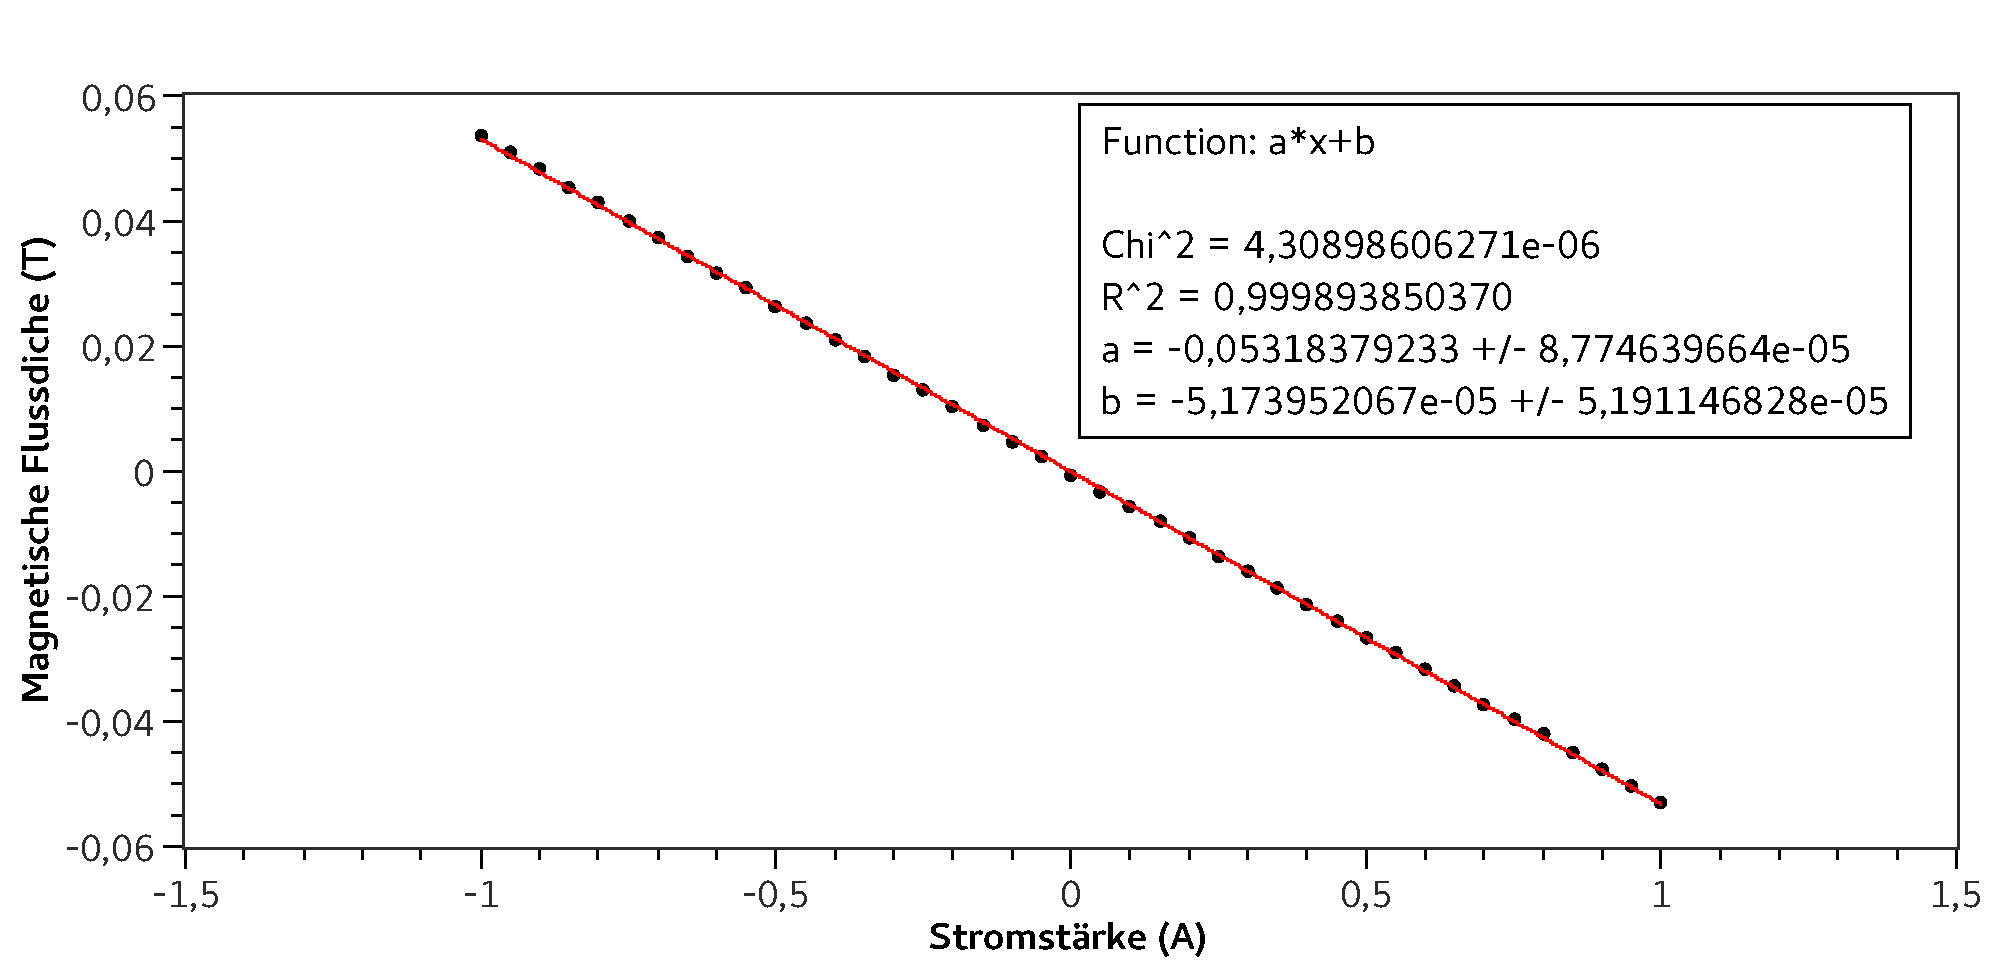
\includegraphics[width=1\textwidth]{fig_spule}
		\centering
		\caption{Die gemessene senkrechte magnetische Flussdichte $B$ ist gegen den Betriebsstrom der Spulen aufgetragen. Die Unsicherheiten sind kleiner als die Symbolgröße.} 
		\label{fig_spule}
		\centering
	\end{figure}

	\subsubsection{Messung der Hysteresekurve}
	Aus der Einführung ist bekannt, dass die Lichtintensität nach dem Analysator proportional zur Magnetisierung ist.
	Die Stärke des magnetischen Felds ergibt sich aus dem in \cref{ss_spule} bestimmten Proportionalitätsfaktor und aus dem Strom, der durch die Spulen fließt.

	Die erste durchgeführte Messung wird verworfen, weil keine eindeutigen Trends in der Messung festzustellen sind, da die Messwerte der relativen Intensität scheinbar willkürlich über den gesamten Messbereich des Magnetfelds schwanken.
	Da dies auf das Umgebungslicht zurückgeführt wird, wird die Messung bei abgedunkeltem Raum wiederholt, was eine Auflösung der Flanken der Magnetisierungsänderung erlaubt.
	Des Weiteren wird beobachtet, dass die Messwerte der Photodiode um ca. $\SI{\pm0,2}{}$ schwanken, wenn man an den Tisch stößt.

	Die so gemessene Hystereseschleife ist in \cref{fig_magn_licht} dargestellt.
		
	\begin{figure}[H] 
		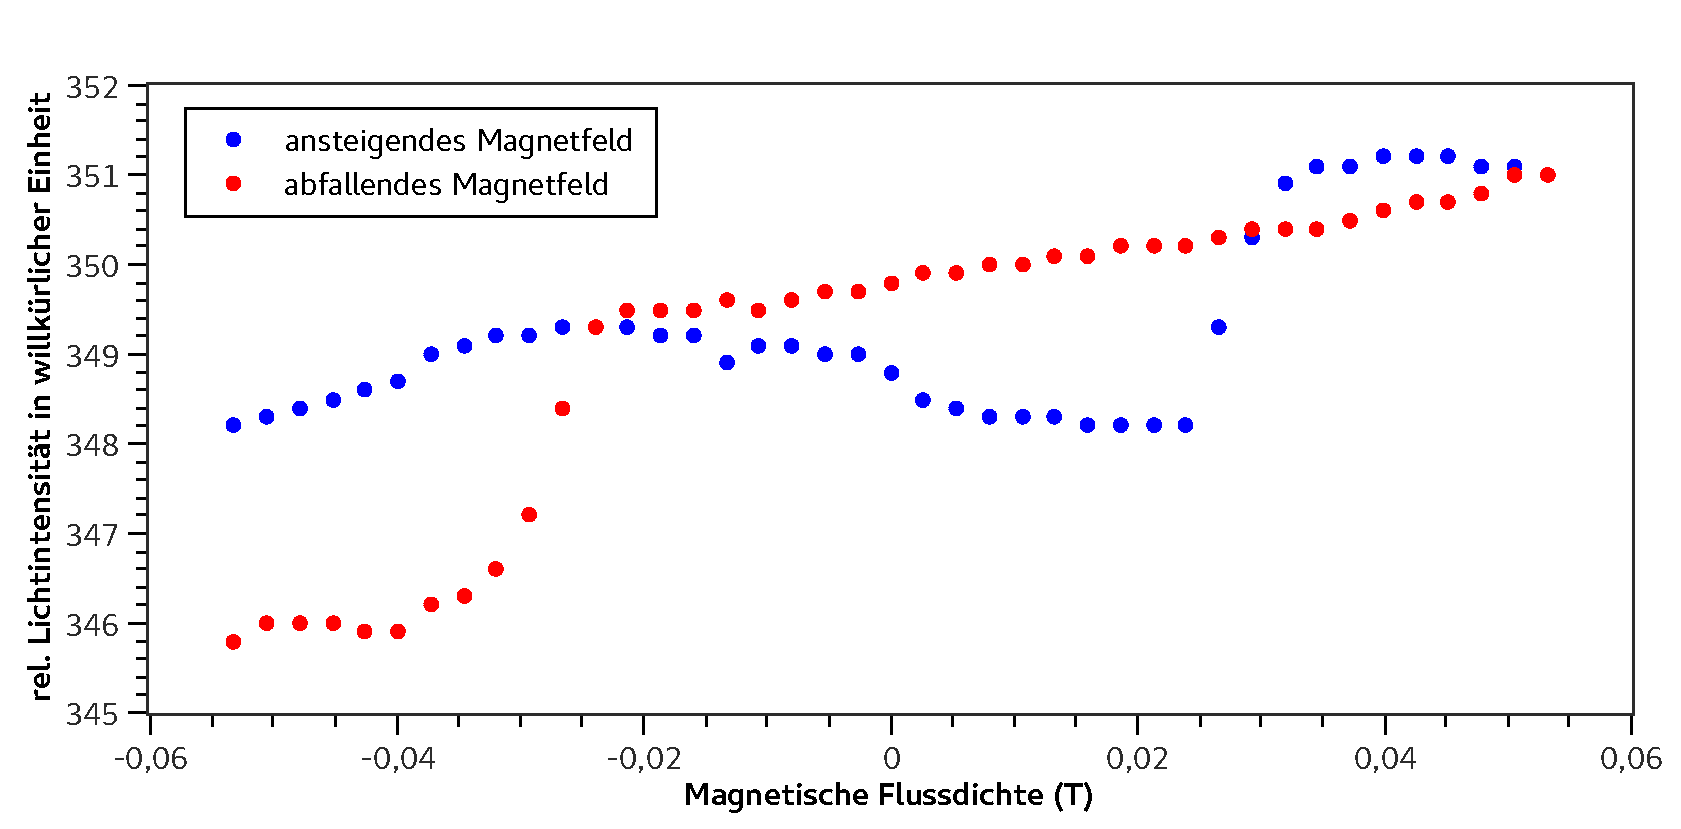
\includegraphics[width=1.00\textwidth]{fig_magn_licht} 
		\centering
		\caption{Die gemessene relative Lichtintensität, die nach dem Analysator gemessen wird, ist gegen die magnetische Flussdichte aufgetragen. 
		Zunächst wurde ein negatives Magnetfeld angelegt. 
		Dieses wird bis auf \SI{0,06}{T} gesteigert.
		Dabei ergibt sich die blaue Messkurve.
		Von \SI{0,06}{T} wird das Feld wieder auf \SI{-0,06}{T} gesenkt und die rote Messkurve aufgezeichnet.
		Die Unsicherheiten sind kleiner als die Symbolgröße.} 
		\label{fig_magn_licht}
		\centering
	\end{figure}

	Die Messkurve wurde in zwei normierte Messabschnitte aufgeteilt.
	Diese sind in \cref{fig_magn1} und \cref{fig_magn2} abgebildet.
	Vor der Messung in \cref{fig_magn1} wird ein negatives Magnetfeld angelegt und dann die Veränderung der Magnetisierung bei steigendem Magnetfeld aufgezeichnet.
	Es zeigt sich ein scheinbarer Anstieg der Magnetisierung in einem Bereich von \SI{-0,02+-0,02}{T}. 
	Dieser fällt allerdings wieder auf den bereits bei \SI{-0,055}{T} gemessenen Wert von ca. \SI{-1}{} zurück.
	Bei \SI{0,03+-0,001}{T} ist ein deutlicher Sprung in der Magnetisierung zu erkennen. 
	Dies ist die Koerzitivfeldstärke. 
	Bei noch stärkeren Magnetfeldern scheint sich die Magnetisierung in Sättigung zu gehen.

	Direkt im Anschluss wird die Messung für ein abnehmendes Magnetfeld durchgeführt.
	Das Ergebnis ist in \cref{fig_magn2} dargestellt.
	Nach einem langsam linearen Abnehmen der Magnetisierung zeigt sich ein deutlich steilerer Abfall bei einer Koerzitivfeldstärke von \SI{0,026+-0,02}{T}. 
	

	\begin{figure}[H]  
		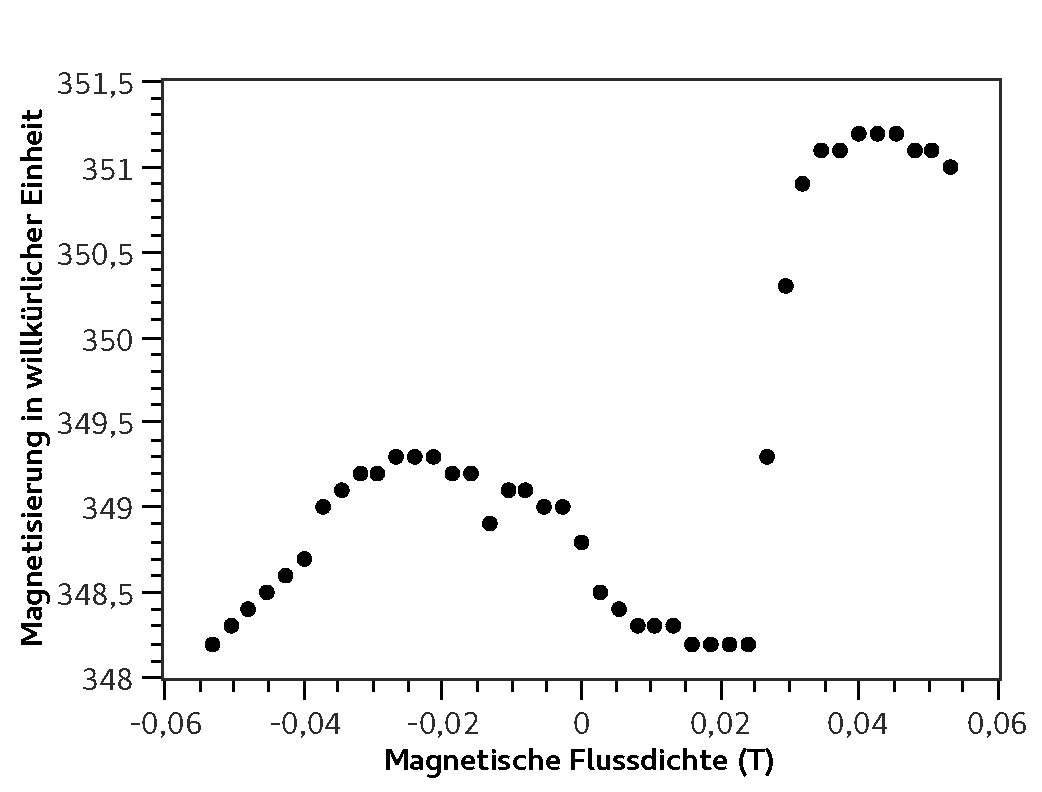
\includegraphics[width=0.90\textwidth]{fig_magn1} 
		\centering
		\caption{Die normierte Magnetisierung der Co/Pt-Probe, die durch die Messung der Polarisationsänderung des einfallenden linear polarisierten Lichts gemessen wird, ist gegen die magnetische Flussdichte aufgetragen. 
		Die Achse ist so normiert, dass die Sättigungsmagnetisierung 1 bzw. -1 beträgt.
		Zunächst wurde ein negatives Magnetfeld angelegt. 
		Dieses wurde bis auf Null abgeschwächt und dann ins Positive gesteigert. 
		Die Unsicherheiten sind kleiner als die Symbolgröße.} 
		\label{fig_magn1}
		\centering
	\end{figure}
	
	\begin{figure}[H] 
		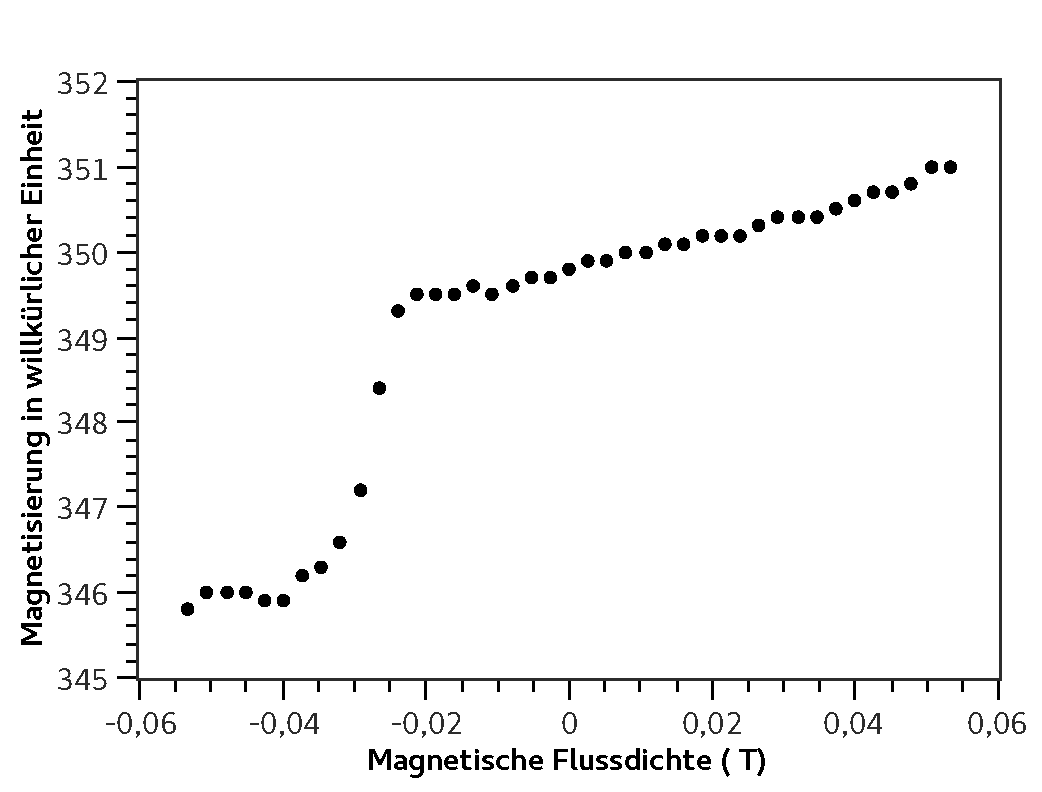
\includegraphics[width=0.90\textwidth]{fig_magn2}
		\centering
		\caption{Die normierte Magnetisierung der Co/Pt-Probe, die durch die Messung der Polarisationsänderung des einfallenden linear polarisierten Lichts gemessen wird, ist gegen die magnetische Flussdichte aufgetragen. 
		Die Achse ist so normiert, dass die Sättigungsmagnetisierung 1 bzw. -1 beträgt.
		Zunächst ist ein positives Magnetfeld angelegt. 
		Dieses wird bis auf Null abgeschwächt und dann in die umgekehrte Richtung erhöht.
		Die Unsicherheiten sind kleiner als die Symbole.} 
		\label{fig_magn2}
		\centering
	\end{figure}
	\subsection{Diskussion}

	Aus \cref{fig_spule} lässt sich die vermutete Proportionalität zwischen magnetischer Flussdichte und Stromstärke durch die Spulen eindeutig ablesen.
	
	\crefrange{fig_magn1}{fig_magn2} weisen die charakteristischen Flanken der starken Magnetisierungsänderung ab einer bestimmten Gegenfeldflussdichte auf.
	Die erwartete Symmetrie der Kurven ist jedoch, wie in \cref{fig_magn_licht} zu erkennen ist, nur begrenzt gegeben.
	Dass die Magnetisierung erst bei einer Koerzitivfeldstärke wieder Null erreicht, lässt sich erkennen und die Koerzitivfeldstärke liegt auch bei beiden Messrichtungen betragsmäßig bei dem gleichen Wert.
	Die Symmetrie wird allerdings unter anderem dadurch gebrochen, dass die Sättigungsmagnetisierung nicht bei beiden Richtungen der Magnetfeldänderung am negativen Ende der Messung der magnetischen Flussdichte gleich ist.
	Dies kann durch Änderungen der Beleuchtungssituation des Raumes durch den sich bewegenden Vorhang sowie die fortschreitende Tageszeit zustande gekommen sein. %TODO Tageszeit ist glaub unwahrscheinlich aber ok
	Es ist außerdem fraglich, ob die Sättigungsmagnetisierung mit der verwendeten Feldstärke erreicht wurde, da die Magnetisierung ober- und unterhalb der Koerzitivfeldstärke nicht konstant ist.
	Außerdem ist in \cref{fig_magn1} ein Maximum unterhalb der Koerzitivfeldstärke.
	Dies widerspricht den Erwartungen und ist vermutlich darauf zurückzuführen, dass während der Messung die Tür des Raums geöffnet wurde und durch diese zusätzliches Licht in den Raum fiel.
	Außerdem bewegte sich durch den Wind der Vorhang, der das Fenster verdunkelte, was ebenfalls für diese Abweichung gesorgt haben kann.%TODO Wind oder Luftzug oder Thermodynamik
	
	Zusätzliche Abweichungen können durch die Empfindlichkeit des Versuchsaufbaus gegen Änderung der Belastung des Tisches.
	So führte ein Aufstützen auf dem Tisch bereits zu einer Intensitätsänderung.
	
	\section{Schlussfolgerung}
	Es konnten die beiden Hypothesen im Wesentlichen nachgewiesen werden.
	Die Annahme, dass die magnetische Flussdichte linear mit dem Stromfluss durch die Spulen zunimmt, konnte eindeutig bestätigt werden.
	
	Die Charakteristiken der Hysteresekurve konnten teilweise gemessen werden.
	Teilweise zeigten sich jedoch auch unerwartete Effekte, die auf nicht hinreichend kontrollierte Umgebungseinflüsse zurückgeführt wurden.
	Deshalb lässt sich sagen, dass für eine präzisere Messung der Hysteresekurve eines Cobalt/Platin-Schichtsystems die gewählte Vorgehensweise prinzipiell zielführend ist, aber einige Anpassungen vorgenommen werden sollten.
	So würde eine zuverlässigere Abdunklung des Versuchsraums zu verlässlicheren Messergebnissen führen. %TODO Wortwiederhohlung lul
	Im konkreten Fall hätte dies bedeutet, dass der Vorhang durch eine windunabhängige Abdunklung wie Rollläden ersetzt würde und dass die Tür während der Versuchsdurchführung geschlossen bleibt.%!
	
	Außerdem könnte man, anstatt den Analysator konstant auf \SI{45}{\degree} einzustellen und das Gesetz von Malus als linear zu nähern, mit dem Analysator jeweils das Maximum der Transmission suchen und so bei der Bestimmung der Magnetisierung eine angenäherte Proportionalität weniger haben, da in diesem Fall die Polarisationsänderung direkt gemessen werden würde. %TODO approven, hmm "Das Messsignal ist die
	%	Lichtintensität, die ein Maß für die (relative) Änderung der Polarisa-
	% 	tion nach Reflexion an der Probe ist, und damit nur proportional zur
	%	Magnetisierung" - Unterschied realtive und nicht realtiv?
	%	Mir ist nur unklar inwiefern sich das von den Einheiten plotten lassen würde wenn man die Winkeländerung nimmt
	%	Außérdem denke ich, dass die Änderung wirklich sehr gering sind ( sonst wäre ja auch die cos^2 linear argumentation rip und des von hand zu optimieren ist wahrscheinlich net möglich) 
	%\printbibliography
\end{document}
